\documentclass{article}
\usepackage{geometry}
 \geometry{
 a4paper,
 total={170mm,257mm},
 left=20mm,
 top=20mm,
 }
\usepackage{tgheros}
\usepackage[utf8]{inputenc}
\usepackage[english]{babel}
%\usepackage[english]{isodate}
%\usepackage[parfill]{parskip}
\usepackage[hybrid]{markdown}
\markdownSetup{
  pipeTables,
  tableCaptions,
  rendererPrototypes = {
    image = {\begin{center}\setkeys{Gin}{width=.99\linewidth}\includegraphics{#2}\end{center}}, % center images inline expanding to page width
    codeSpan = {\texttt{#1}}, % Render inline code via `\texttt`.'
  }
}
\title{
  \textbf{AmpliPro Streamer Unit - User Manual}
}
\date{ \textbf{ Version: 0.3.5}}
\setlength\parindent{0pt}
\begin{document}

\maketitle
\setkeys{Gin}{width=.99\linewidth}
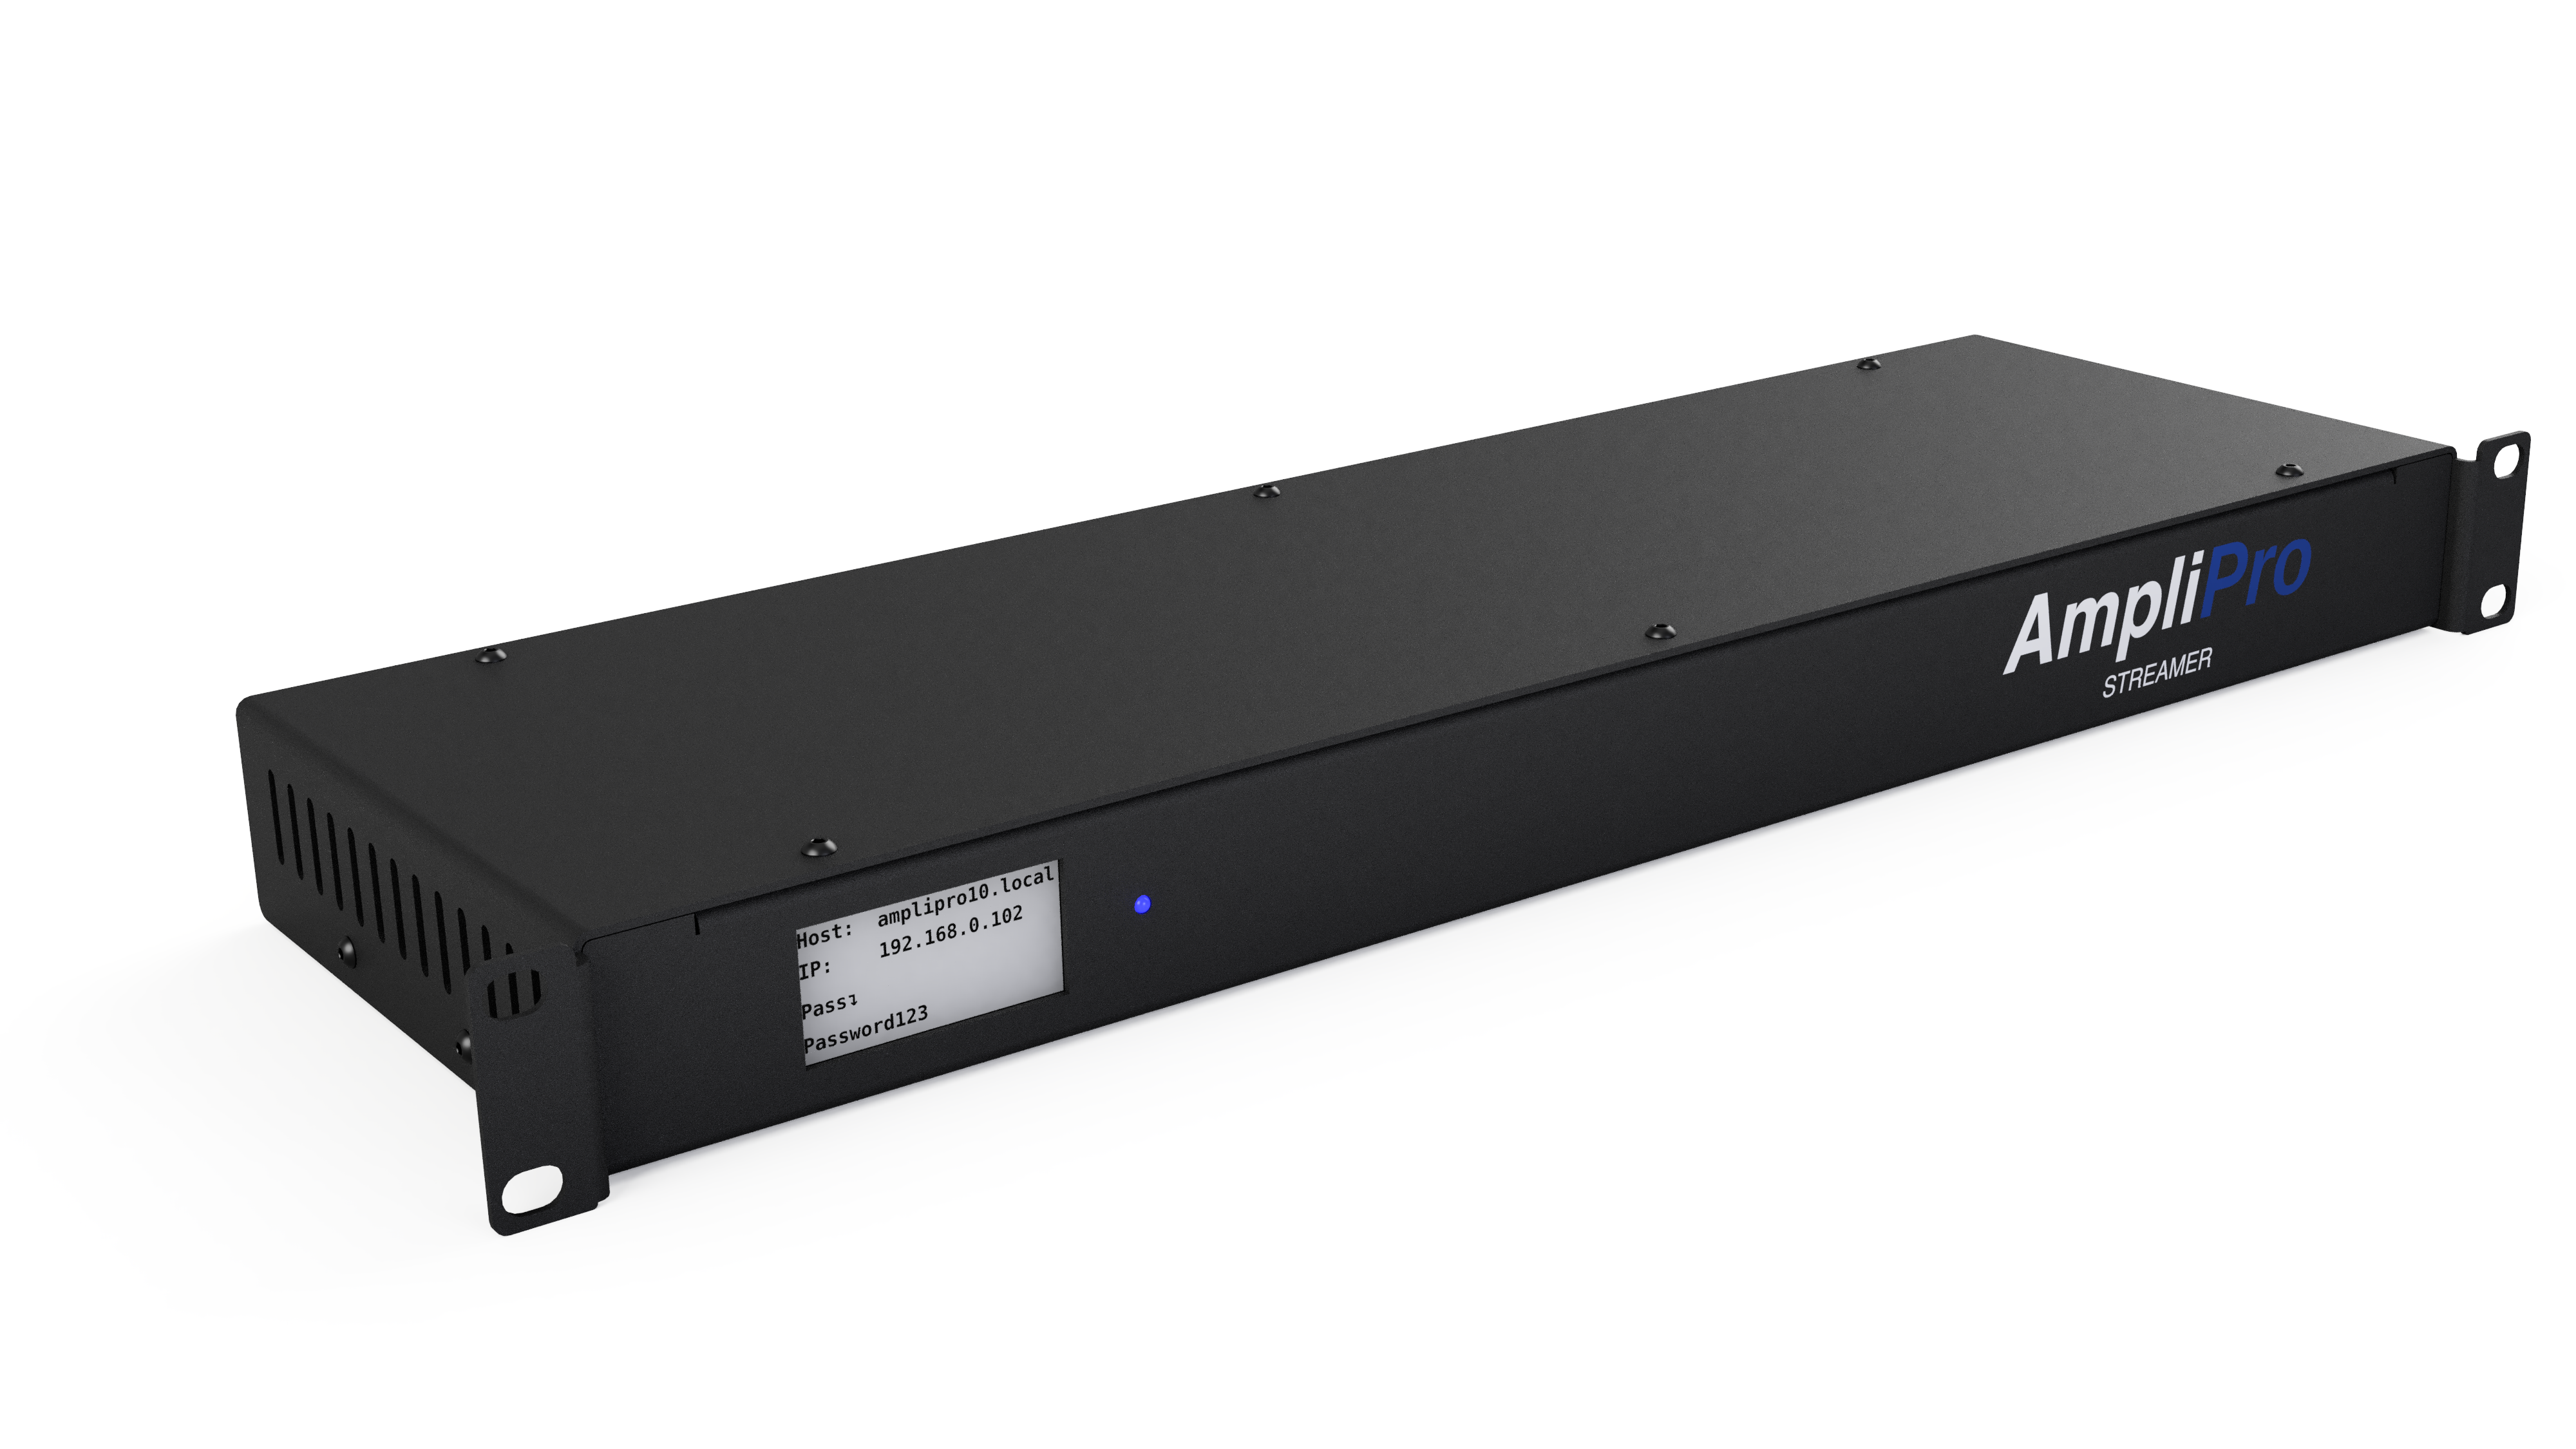
\includegraphics{ streamer/AmpliPro_streamer_front_angled.png}
\newline
\newline
\begin{center}
  \LARGE{ \textbf{ Device Model: AP1-S4}}
\end{center}

\includegraphics{ imgs/MicroNova_Logo.jpg}

\newpage
\tableofcontents
\newpage
\pagenumbering{arabic}

\markdownInput{streamer/LINKS.md}
\newpage
\markdownInput{common/SAFETY.md}
\newpage
\markdownInput{common/FCC.md}
\newpage
\markdownInput{streamer/OVERVIEW.md}
\newpage
\markdownInput{streamer/STREAMER_SPECS.md}
\newpage
\markdownInput{streamer/INSTALLATION.md}
\newpage
\markdownInput{common/TROUBLESHOOTING.md}
\newpage
\markdownInput{common/WARRANTY.md}

\end{document}
